%A pointform description of the general idea
%\begin{itemize}
%	\item A D-NURBS approach to simulation. Use a Jacobian to map from UV positions in a NURBS parametric space to world space positions on the surface. 
%	\item \textbf{Shape Matching}: From the sample world space positions on a single NURBS surface, we solve a least squares problem to fit a \textit{projection operator} to the surface. This projection operator maps monomials in the undeformed space, to the least squares estimate of the deformed positions for the given monomials.
%	\item With DNURBS and Shape Matching VEM we have two mappings: a UV to undeformed world space with our NURBS Jacobian, then an undeformed to deformed mapping with the projection operators. This lets us form a set of generalized coordinates in terms of our control points of the NURBS surface (section 1.4).
%	\item For an arbitrary position in space (not necessarily on the surface), we can build a projection operator unique to this point via a weighted sum of the projection operators of the projection operators for each NURBS (eq 5). From this we can reconstruct an estimate of the deformed position from the monomial basis defined using its undeformed position.
%	\item For any point in space, we need to compute a set of weights to the projection operators defined on the surfaces with the following criteria: the weights sum to 1, are nonzero, and depend on the distances to the surfaces (See section 1.8).
%	\item With this mapping for undeformed to deformed positions, this yields a simple definition for the deformation gradient (eq 12).
%	\item Armed with our deformation gradient, we next define the Lagrangian, but this basic form isn't sufficient. We augment our kinetic and potential energies with a stability term (ref VEM). This accounts for cases in which the position of the nodal values don't match their estimated positions defined by the projection operator mapping.
%	\item \textbf{Raycasting Quadrature}: To compute the volume integrals we make use of raycasting quadrature approach (ref) where we uniform sample a YZ grid and shoot rays in the X direction. We then use the points of intersection to define integrations bounds for 1D integrals along these rays, which we integrate numerically.
%	\item With our augmented lagrangian, we use the Euler-Lagrange equation to arrive at equations of motion. Our generalized coordinates give us direct updates on the control points of the NURBS. Currently we are using linearly-implicit Euler for time integration.
%	\item \textbf{Handling trimmed NURBS}: For this case we update the original control points, but we must only sample points within the boundary. To compute these points we use an approach similar to the raycasting quadrature but in 2D. In the paremtric domain for a T-NURBS we sample uniforly in the V direction and shoot rays along the U axis. At each region of intersection, we sample more values along the ray. The final result is a set of UV coordinates that respect the boundary defined by NURBS curves.
%\end{itemize}
\section{Overview}
The input to the Shape Matching Element Method (SEM)  is a NURBS \emph{boundary representation} of a volumetric object, along with a set of physical parameters 
(density, constitutive model, model parameters etc). 
The boundary representation is composed of one or more (not necessarily explicitly connected) NURBS surface primitives that we will call \emph{parts}.
The output is an elastodynamic simulation. 
SEM consists of preprocessing and runtime simulation phases (~\refalg{sem_preprocess}, ~\refalg{sem_simulation}) and at no point do we need to generate a volumetric mesh of the input. 
In the \emph{preprocessing} stage we use raycasting to find quadrature points and weights for volumetric integration, as well as to compute part blending parameters. 
Finally we construct local shape matching operators and construct the mass matrix for our problem. 

At runtime we use standard time integration schemes to time step the system. 
This requires us to evaluate the energy, gradient and Hessian (implicit only) which we do at the previously computed quadrature points. 
For collisions we use penalty forces and apply them as external forces during integration (though other methods could be used).

\begin{algorithm}[h]
	\begin{algorithmic}[1]
		\Procedure{Preprocess}{$model$}
		\State{// Get initial DOF and sample boundary  \Comment{Section \ref{sec:geometric_model}}}
		\State $\vc{q} \gets \text{GetControlPoints}(model)$
		\State $\samp{\Jnurbs}, \wt \gets \text{SampleNURBS}(model)$
		\State $\vc{x^0} \gets \wt \samp{\Jnurbs} \vc{q}$
        \Statex
      
    	\State{// Generate material points inside the model}
		\State $\st{X} \gets \text{RaycastQuadrature}(model)$ \Comment{Section \ref{sec:quadrature}}
		\Statex   
		
		\State{// Set of blending weights for each $\refX \in \st{X}$} 
     	\State $\st{W} \gets \text{BlendingWeights}(model, \st{X}, \alpha)$    \Comment{Section \ref{sec:weights}}
		\Statex
		\State $\XBs \gets \text{DeformationOrigins}(\st{X}, \st{w})$  \Comment{Section \ref{sec:origins}}
		\Statex
		
		\State{// Create projection operator}
		\State $\Pi \gets \text{ShapeMatching}(\vc{q}, \samp{\Jnurbs}, \st{\wt}, \XBs)$ \Comment{Section \ref{sec:shapematching}}
		\Statex
		
		\State{// Form mass matrix and error hessian, respectively}
    	\State $\MM \gets \text{MassMatrix}(\st{X}, \XBs, \st{W},\Pi)$    \Comment{Section \ref{ssec:mass_matrix}}
     	\State $\ME \gets \text{ErrorMatrix}(\vc{x^0}, \XBs, \st{W},\Pi)$  \Comment{Section \ref{ssec:error_energy}}
	\EndProcedure
\end{algorithmic}
\caption{Shape Matching Element Preprocessing}
\label{alg:sem_preprocess}
\end{algorithm}

%\section{Methods}
\section{Geometric Model}
\label{sec:geometric_model}

Our algorithm acts on objects composed of multiple NURBS surfaces~(\reffig{NURBS}).
\begin{figure}[h]
    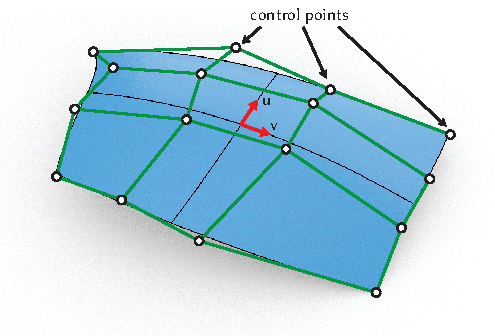
\includegraphics[width=\columnwidth]{figures/nurbs_patch}
    \caption{A cubic NURBS patch with 16 control points.}
    \label{fig:NURBS}
\end{figure}
The three-dimensional position, $\defX$, of any point on a NURBS surface can be written as 
\begin{equation}
\label{eqn:nurbs_srf}
\defX\left(u,v\right) = \sum_{i=1}^n\sum_{j=1}^m \phi_{ij}\left(u,v\right)\vc{q}_{ij},
    %\mathbf{x}(u,v) = \frac{\sum_{i=1}^{n}\sum_{j=1}^{m}  \mathbf{p}_{i,j} w_{i,j} B_{i,k}(u)B_{j,l}(v)}
    %{\sum_{i=1}^{n}\sum_{j=1}^{m} w_{i,j} B_{i,k}(u)B_{j,l}(v)}
    %\text{,}
\end{equation}
where $u$ and $v$ $\in \real$ are the coordinates in the 2D parametric domain, $n$ and $m$ are the number of control points in the $u$ and $v$ directions, $\mathbf{q}_{ij}\in\real^3$ are the control points and $\phi_{ij}\left(u,v\right)\in\real$ are the NURBS
basis functions given by 
\begin{equation*}
    \phi_{ij}\left(u,v\right) = \frac{\omega_{i,j}\beta_{ik}(u)\beta_{jl}(v)}{\sum_{r=1}^{n}\sum_{s=1}^{m} \omega_{ij} \beta_{ik}(u)\beta_{jl}(v)},
\end{equation*} where $\beta_{ik}$ (resp. $\beta_{jl}$) is the $i^{th}$ ($j^{th}$) B-spline basis of order $k$ ($l$).

Exploiting linearity with respect to the control points, we can express this mapping as
\begin{equation}
    \defX\left(u,v\right) = \underbrace{\begin{pmatrix} \phi_{11}\left(u,v\right)\ident & \dots & \phi_{nm}\left(u,v\right)\ident \end{pmatrix}}_{\Jnurbs\left(u,v\right)}
    \underbrace{\begin{pmatrix} \vc{q}_{11} \\ \vdots \\ \vc{q}_{nm}\end{pmatrix}}_{\vc{q}},
\end{equation} where $\Jnurbs\left(u,v\right)$ is the NURBS Jacobian, $\ident$ is the $3\times3$ identity matrix and $\vc{q}$ is the vector of generalized coordinates~\cite{lanczos2012variational}
The Shape Matching Element Method will follow from this kinematic description.

\section{Shape Matching}
\label{sec:shapematching}

We begin by describing shape matching to a single NURBS part. 
Given two different configurations of the same part (specified by the control points), shape matching computes a polynomial deformation that best aligns them.

Let $\vc{q^0}$ be the initial control points of the part, provided by the modeler, and $\vc{q}$ be a vector of modified control point values.
We can compute the undeformed (or reference) position of any point on our part using $\refX\left(u,v\right) = \Jnurbs\left(u,v\right)\mathbf{q^0}$ and the corresponding
deformed (world space) position as $\defX\left(u,v\right) = \Jnurbs\left(u,v\right)\mathbf{q}$.

We can define a polynomial deformation from $\refX = \begin{pmatrix} X & Y & Z \end{pmatrix}^T$ to $\defX$  as 
\begin{equation}
    \defX\left(\refX\right) = 
    \underbrace{\begin{bmatrix}
    \mathbf{p}^T(\refX-\bar{\refX}) & \mathbf{0} & \mathbf{0} & 1 & 0 & 0\\
    \mathbf{0} & \mathbf{p}^T(\refX-\bar{\refX}) & \mathbf{0} & 0 & 1 & 0\\
    \mathbf{0} & \mathbf{0} & \mathbf{p}^T(\refX-\bar{\refX}) & 0 & 0 & 1\\
    \end{bmatrix}}_{\Pmatx}
    \Pcox,
    \label{eq:projection}
\end{equation} where $\mathbf{p}^T\left(\refX\right)$ is the polynomial basis vector \newline (eg $\begin{bmatrix} X & Y & Z & X\cdot Y & X\cdot Z & Y\cdot Z& X\cdot X & Y\cdot Y & Z\cdot Z \end{bmatrix}$ ),
$\bar{\refX}$ is an a priori chosen origin around which to deform, $\Pco$ are the coefficients for the 
non-constant part of the polynomial and $\tr$ is the translation of the deformation origin. 
We can compute the shape matching deformation by solving~\cite{10.1145/1073204.1073216}
\begin{equation}
   \Pcox^* = \arg\min_{\Pco,\tr} \int \left\lvert\left\lvert\Pmatx\Pcox - \Jnurbs\vc{q}\right\rvert\right\rvert^2_2 dudv,
\end{equation} where we have suppressed the dependence of $\refX$ and $\Jnurbs$ on $u$ and $v$ for the sake of brevity.

We discretize the shape matching energy and minimize by solving
\begin{equation}
\samp{\Pmat}^T\wt\samp{\Pmat}\Pcox = \samp{\Pmat}^T\wt\samp{\Jnurbs}\vc{q}.
\label{eq:shapematch}
\end{equation} Here $\samp{\Pmat}$ (resp. $\samp{\Jnurbs}$) is a $3s \times 3(k+1)$ (resp. $3s \times 3nm$) matrix where $s$ is the number of quadrature points, 
$k$ is the number of  terms in the shape matching polynomial and $3nm$ is the number of NURBS control points. 
$\samp{\Pmat}$ (resp. $\samp{\Jnurbs}$) is constructed by stacking the evaluations of $\Pmatxuv$ (resp. $\Jnurbs\left(u, v\right)$) at each
quadrature point.
$\wt$ is a diagonal, $3s \times 3s$ matrix of integration weights.

Quadrature points are selected so that $\samp{\Jnurbs}$ is of sufficient rank required to represent all control points. We achieve this by sampling over each knot span defined by the  B-splines, and find it effective to use the order of the NURBS as the number of quadrature points sampled in each knot span.
\ty{the number of samples may be different if order in the u direction and v differ, but I figured it was best to keep this simple.}

\nicetohave{now I do want that shape matching figure showing constant, linear and quadratic matching}

\paragraph*{Relationship to the Virtual Element Method}
For a non-planar NURBS part, and given a sufficient number of quadrature points, ~\refeq{shapematch} will be well-posed allowing us to write: $\Pcox^* = \Pi\vc{q}$ where
\begin{equation*}
    \Pi = \left(\samp{\Pmat}^T\wt\samp{\Pmat}\right)^{-1}\samp{\Pmat}^T\wt\samp{\Jnurbs},
\end{equation*} is a projection from the space of control points onto the space of polynomials. 
This projection serves an identical purpose (and is mathematically equivalent up to choice of metric) to the projection operator used in VEM~\cite{10.1142/S021820251440003X}.
VEM uses a single polynomial projection per polyhedral element to solve differential equations on complex volumetric meshes.
We interpret shape matching as converting our NURBS part into a single Virtual Element suitable for elastodynamics simulation.
Unfortunately, a single polynomial deformation space will not be suitably expressive for even moderately complex models.
Previous work~\cite{10.1145/1073204.1073216,10.1145/1275808.1276480} used additional lattices or partitions of the reference space to 
increase the number of polynomials in the shape matching. In contrast, our meshless Shape Matching Element Method which works directly on the NURBS
geometry itself.

\section{Shape Matching Element Method}
 Each input object is composed of a set of boundary representations, $\Prts$, one for each part $\prt\in\Prts$. 
 Our kinematic mapping is a blended construction~\cite{10.1145/2614028.2615427,blendedFORKS2016} which we write as

 \begin{equation}
    \defX\left(\refX\right) = \sum_{\prt_i\in\Prts} \bldxi\Pmatxi\Pi_i\vc{q}_i, 
    \label{eq:kinematics}
 \end{equation} where $\bldxi$, $\Pmatxi$, $\Pi_i$ and $\vc{q}_i$ are the blending weights, polynomial basis, projection operator and control points for the $i^{th}$
 part respectively.  
 \ty{I'm wondering if we should add a line emphasizing that while we linearly blend, the resulting deformation map is a nonlinear map unique to each X. But maybe this obvious}
 
 \subsection*{Multiple Part Projection}
As in ~\refsec{shapematching} we construct each $\Pi_i$ via shape matching. 
It is tempting to use an identical polynomial basis matrix, $\Pmatx$ for all parts, $\prt_i$, but recall that constructing $\Pmatx$ requires the selection of a deformation
origin $\bar{\refX}$~(\refeq{projection}). 
Using the same origin for all polynomials limits the expressivity of the kinematic model~\cite{STBS:2011}.
Instead we choose a set of points $\XBs$ ($0 < |\XBs| < |\Prts|$) to act as deformation origins~(\refsec{origins}).
For each part we now construct $\Pmatxi$ using its associated deformation origin $\bar{\refX}_j\in \XBs$, where each origin can
be shared between multiple parts.

Attempting to use $\Pmatxi$ in~\refeq{shapematch} on a per-part basis is problematic as it can become ill-posed, especially for planar boundary representations. 
To alleviate this problem we invoke the \emph{hierarchical ordering principle}, which argues that the behavior of a system is typically 
dominated by lower order effects~\cite{li2006regularities}. 
Mechanically, this principle suggests that the amount of motion modelled by increasingly high-order polynomials is, itself, decreasing. 
This implies that we can achieve acceptable shape matching results by performing shape matching hierarchically -- starting with the constant term and then 
fitting the remaining deformation with progressively higher-order expressions. 

For a given part, $\prt_i$, with associated origin $\bar{\refX}_j$ we first estimate the constant term, $\tr_i$ as the centroid of all parts associated with $\bar{\refX}_j$.
Next we fit the linear part of the deformation by performing linear shape matching to $\prt_i$. 
This can be repeated for polynomials of arbitrary high order, for instance here we apply this approach to quadratic shape matching:

\begin{equation}
    \begin{split}
        \tr_i  & = \sum_{\prt_k \in \bar{\refX}_j} \underbrace{\mathbbm{1}^T\wt_k \samp{\Jnurbs}_k}_{B_{ik}}\vc{q}_k \\
        \vc{c}_i^1 & = \smash{\underbrace{\left(\samp{\Pmat^1}^T\wt_i\samp{\Pmat^1}\right)}_{A^1_i}}^{-1}\bigg(\underbrace{\samp{\Pmat^1}^T\wt_i\samp{\Jnurbs}_i}_{B^1_i}\vc{q}_i-\underbrace{\samp{\Pmat^1}^T\wt_i\mathbbm{1}}_{T^1_i}\tr_i\bigg)\\
        \vc{c}_i^2 & = \smash{\underbrace{\left(\samp{\Pmat^2}^T\wt_i\samp{\Pmat^2}\right)}_{A^2_i}}^{-1}\bigg(\underbrace{\samp{\Pmat^2}^T\wt_i\samp{\Jnurbs}_i}_{B^2_i}\vc{q}_i-\underbrace{\samp{\Pmat^2}^T\wt_i\samp{\Pmat^1}}_{D^2_i}\vc{c}_i^1 - \underbrace{\samp{\Pmat^2}^T\wt_i\mathbbm{1}}_{T^2_i}\tr_i\bigg)
    \end{split},
    \label{eq:hfit} 
\end{equation} where $\Pmat^l$ contains only the monomial basis of order $l$,  $\samp{\Pmat^l}$ is the stacked evaluation of this matrix at the $s$ quadrature points and $\vc{c}^l_i$ are the corresponding coefficients. 
Finally, $\wt_i$ is the diagonal integration weight matrix and $\mathbbm{1}\in\real^{3s\times3}$ is a matrix of stacked $3\times3$ identity matrices -- one for each quadrature point.

\begin{figure}[h]
    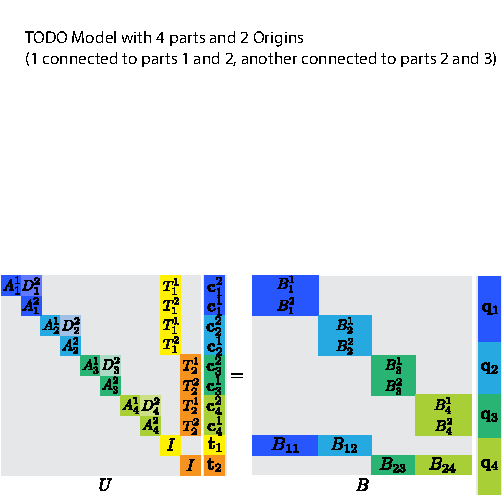
\includegraphics[width=\columnwidth]{figures/projection_operator_solve}
    \caption{A simple, four part model with two deformation origins and the corresponding matrix equation for the quadratic coefficients.}
    \label{fig:multiparts}
\end{figure}

%%single projector for every object
When assembled for all parts,~\refeq{hfit}, yields a block upper triangular matrix $U$ and a sparse matrix $B$ ~(\reffig{multiparts}) which can be used to efficiently to compute the projection 
operator for the entire object $\Pi = U^{-1}B\vc{q}$. 
The structure of $U$ and $B$ ensures that $\Pi$ only couples objects which share deformation centers, which implies a sparse $\Pi$. 
The per-part projection operators $\Pi_i$ correspond to blocks of rows of $\Pi$. 
Coupling via the deformation origins ensures our method will reproduce rigid and linear deformations in regions around these points, while higher order 
terms help compensate for more local deformations.

\dave{should have done Chebyshev shape matching to ensure higher order terms are orthogonal which would gaurantee exact reconstruction}

\subsection{Meshless Blending Weight Computation}
\label{sec:weights}
% \dave{Desireable Properties}
% \dave{Construction via post normalization}
% \dave{only need blending weights at quadrature points and surface samples so given sparse set of quadrature points compute blending weights using raycasting}
% \dave{things to explain (1) raycasting works for overlapping geometric, seperated geometry (2) weights glue objects together}
% \dave{maybe but weight figure here so reviewers immediately know that it looks pretty good}
% \dave{need to mention Monte Carlo Geometry processing but can't use it because our parts can overlap and that's a tricky boundary condition}

Our kinematic map~(\refeq{kinematics}) requires blending weights in order to homogenize our per-part representation. 
Specifying weights manually would be antithetical to our goal of providing a seamless translation from surface representation to physics-based animation.
Automatic  weight computation is well-studied (see ~\citet{10.1145/2766952,BBW:2011} and ~\citet{10.1145/2010324.1964968}) but typically requires solving 
an optimization problem that itself relies on a volumetric discretization. 
This can be avoided by using stochastic methods~\cite{Sawhney:2020:MCG} but these do not yet support the boundary conditions we require for our problem. 

Ideally our shape functions would both partition unity and obey the Kronecker delta property (the $i^{th}$ blending function is one at $i^{th}$ part and zero on all other parts).
These properties ensure that our simulation can properly represent translation and that the solution stored at each part is the actual deformed position.
Additionally we would like our weights to be sparse both for performance reasons (leads to sparse matrices) and for expressivity (leads to locality of deformation). 

While partition of unity and sparsity are straightforward to enforce, the overlapping and intersecting parts~(\reffig{badmodels}) often encountered in non-engineering models leads
to a contradiction -- how can the blending functions be both one and zero at the points of overlap ? 
Our solution is to allow weights to include bounded discontinuities at these points and it is these discontinuities that are difficult to enforce 
with previous methods. 
\dave{ideally need a didactic figure showing this}

Given a set of reference space points $\st{X}$ inside our model, we want to evaluate $\bld_i\left(\refX_j\right)$, where $\bld_i$ is the weight function associated with 
the $i^{th}$ part, $\prt_i$, and $\refX_j\in\st{X}$. 
For each $\refX_j$ we find the nearest point on $\prt_i$, $\clst$.
We cast a ray from $\clst$, towards $\refX_j$ and find the intersection with the nearest part, $\rhit$.

Using these two distances we define a linear \emph{distance weight} using the well-known ReLU function:
\begin{equation}
\theta_i = \max (1.0 - \frac{d_{\text{primary}}}{\min (d_{\text{total}}, \alpha)}, 0.0)
\text{,}
\end{equation}
where $\alpha$ is a distance cutoff parameter. 
This distance weight~(\reffig{plot_distance_weight}) is the result of interpolating along the ray from $\clst$ to $\rhit$ (or a fixed point that depends on $\alpha$). 
These weights obey the Kronecker delta property for all parts but do not partition unity which we repair using a post-normalization step. For non-planar surfaces, $\rhit$ may lie on the same part as $\clst$. For points inside closed periodic surfaces, it is critical that the weights equal one in this case, so we set $\theta_i = 1$.

% \begin{figure}[h]
%     \centering
%     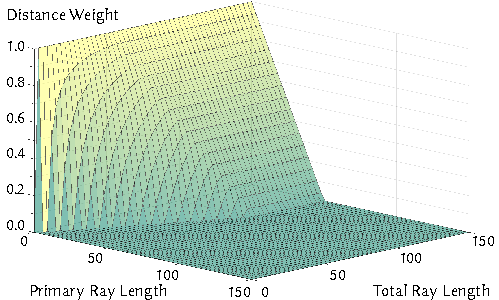
\includegraphics[width=3.33in]{figures/plot_distance_weight.pdf}
%     \caption{We plot the distance weight with respect to the primary and total ray length. Here the cutoff distance is 50.
%     }
%     \label{fig:plot_distance_weight}
%     \vspace{-5pt}
%   \end{figure} 

%\begin{figure}
%    \includegraphics[width=\columnwidth]{example-image-a}
%    \caption{Figure showing how weight calculation works (left) ray casting plus result (right) after correcting for partition of unity}
%    \label{fig:weightcompute}
%\end{figure}

At each $\refX_j$ we want to compute $\mathbf{\bld}(\mathbf{X}_j) =  \left( \bld_1(\mathbf{X}_j), \dots, \bld_n(\mathbf{X}_j) \right)$, where 
$\sum_{i=1}^n\bld_i(\mathbf{X}_j) = 1$, and each $\bld_i \geq 0$, which we enforce by solving a local optimization problem: 

\begin{equation}
\begin{aligned}
\mathbf{w}(\mathbf{X}_j) =  \arg\min_{\mathbf{w}} \quad & \mathbf{w}^T \Theta(\mathbf{X}_j) \mathbf{w}    \\
\textrm{st} \quad & 0 \leq w_i \leq 1 \mbox{ }\forall i                    \\
                  &   \sum_i^n w_i = 1                      \\
\end{aligned}
\end{equation}

where $\Theta(\mathbf{X}) = \text{diag}\left( \frac{1}{\theta_1},\frac{1}{\theta_2},\dots,\frac{1}{\theta_n}\right)$. 

\begin{wrapfigure}[11]{l}{0.31\columnwidth}
    \begin{center}
            %\vspace{-0.7cm}
            %\hspace{-0.1cm}
            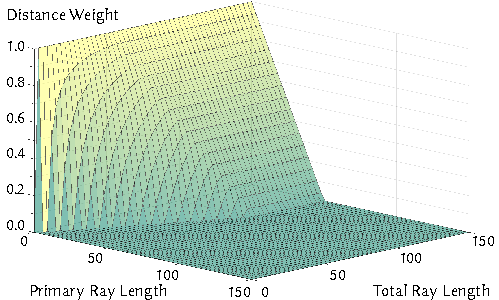
\includegraphics[width=0.3\columnwidth]{figures/plot_distance_weight.pdf}
            
    \end{center}
    \caption{ \label{fig:plot_distance_weight} Distance weight as a function of primary and total ray length with cutoff distance 50.}
  \end{wrapfigure}


This post-process ensures that our blending weights partition unity and are non-negative~(\reffig{distance_weight_puft}). 
For any point on a part that is non-intersecting, the weights will satisfy the Kronecker delta property since the inverse distance weights imply that only
a single $\Theta_i$ will have a non-infinite weight. 
For points that lie on more than one part, the weights associated with the intersecting parts will be equal and all others will be zero
This implies that the deformed positions of these intersecting points will be an average, which is a plausible solution and ensures continuity.
Finally, the distance cutoff $\alpha$ allows us to control the sparsity of the blending weights. We employ a simple heuristic to select $\alpha$ by searching for a $\alpha$ that produces a set of blending weights meeting a desired sparsity target $T \in \left( 0,1\right)$, which is defined as the ratio of non-zeros to total number of weights. This yields a unitless, easy to tune parameter.

\begin{figure}[h]
    \centering
    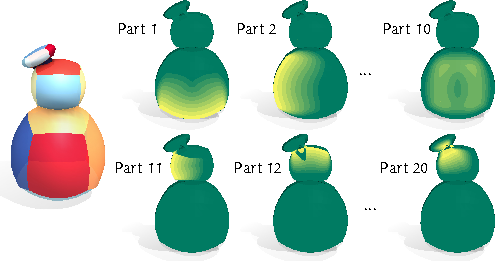
\includegraphics[width=3.33in]{figures/distance_weight_puft.pdf}
    \caption{Our blending weights decay smoothly from 1.0 (yellow) to 0.0 (green) when moving away from its closest surface. Here we visualize the distribution of the distance weights (with cutoff distance 5.0) corresponding to each part.   
    }
    \label{fig:distance_weight_puft}
    \vspace{-5pt}
  \end{figure} 
  %
  %

Using raycasting to compute blending weights imbues our method with similar advantages to \citet{Sawhney:2020:MCG} (allowing us to 
handle intersecting geometry, geometry with gaps and to perform constructive solid geometry operations on the fly),
but allows us to use more general weighting functions and apply the appropriate behavior for intersecting parts.
The price we pay is that our weights are not C0 continuous but rather Lipschitz smooth.
Perturbations in the boundaries of parts can cause bounded jumps in our distance weights. 
However, these jumps occupy an infinitesimal percentage of the volume of our object, and are easy to avoid when integrating
physical quantities, leaving our simulation unaffected. 

\subsection{Choosing Deformation Origins}
\label{sec:origins}
% \dave{Ty: try to follow this formula when writing 
% \dave{maybe this should come after weight computation ?}
% (1) what is the purpose of this part of the method ?
% (2) what are the criteria for success
% (3) what is our assumed input 
% (4) what is the desired output
% (5) what's the algorith,
% (6) add proofs/diagrams/figures that show we satisfy (2). }
Each part, $\prt_i$, must be associated with a single deformation origin, $\bar{\refX}_j$, and each origin is computed as the centroid of the set of parts with which it is associated. 
While we constrain a part to be paired with only one deformation origin, an origin may be associated any number of parts. 

%of the blending weights. Intuitively, this means that for a region in which weights are high for a subset of parts, the origin of deformation should be centered in this region.

\begin{figure}[h]
    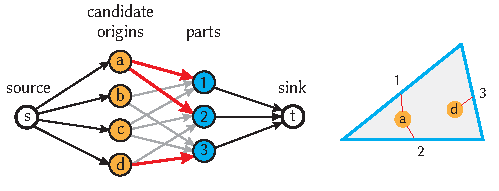
\includegraphics[width=\columnwidth]{figures/origin_network}
    \caption{Example structure for the network flow selection of deformation origins with a shape consisting of three parts. Red arrows indicate each parts origin association. \dave{make it clear edges of triangle are sep. parts, add capacities and costs}}
    \label{fig:network_flow} 
\end{figure}

Candidate deformation origins are selected by clustering quadrature points~(themselves computed in \refsec{quadrature}).
We group quadrature points by the combination of parts influencing each point (non-zero blending weight~(\refsec{weights})).
Each group now represents a unique part combination and the centroids of these groups become deformation origin candidates.
To assign deformation origins to parts we use an integer network flow approach~(\reffig{network_flow}). 

Consider a directed bipartite graph $G=(V = A \cup B,E)$ where each node in $A$ corresponds to a deformation origin candidate and each node in $B$ represents a part. 
$E$ is the set of edges connecting nodes in $A$ to $B$ where each origin has an edge to every part with which it attempts to associate. 
We augment $G$ to form $G'=(V' = A \cup B \cup \{s,t\}, E')$ where $V'$  is the new set of nodes now containing a source, $s$, and sink, $t$. 
$E'$ is the augmented set of nodes connecting $s$ to each candidate in $A$ and connecting each part in $B$ to the sink $t$. 
Each edge $(i,j) \in E'$ has an associated flow $f_{ij}$ and capacity constraint $u_{ij}$, and each edge in $E$ also has a cost $c_{ij}$. 
The principal constraint for this network flow problem is the conservation constraint, meaning that the net flow for all nodes in $V$ is zero.
Each edge from $B$ to $t$ is assigned a capacity of $1$, which enforces that any part node in $B$ receives flow from a single edge, 
and as a consequence each part may only be associated with a single deformation origin. 
The last step is to specify the costs on the edges, $E$, between the deformation origin candidates and the parts. 

Given a quadrature point group, and an edge from the associated deformation origin to $\prt_i$, we set the edge cost to be the sum, 
over all quadrature points in the group of the blending weights associated with $\prt_i$.
This cost penalizes heavily ``connected'' origin candidates, encouraging sparsity during origin selection. 
This amounts to minimizing the following integer linear program:
\begin{equation}
\begin{aligned}
\mathbf{f} =  \arg\min_{\mathbf{f}} \quad & \mathbf{c}^T \mathbf{f}    \\
\textrm{st} \quad & A_{\text{cons}} \mathbf{f} = 0  \\
                  & f_i \in \integer \mbox{ }\forall i	\\
                  & 0 \leq f_i \leq u_i
\end{aligned}
\end{equation}
where $\mathbf{f}$ and $\mathbf{c}$ are the edge flow and cost values, respectively, assembled into vectors, and $A_{\text{cons}}$ forms the set of constraints satisfying the flow conservation constraint. 
We solve this using the dual simplex solver in MATLAB.
%\ty{we use the default in intlinprog, which should be dual-simplex} We choose $\XBs$ to be all the deformation origin candidates in $A$ that have an outgoing flow of at least $1$. 

\subsection{Meshless Integration}
\label{sec:quadrature}
We integrate physical quantities over our undeformed object using raycasting based quadrature~\cite{KHOSRAVIFARD201030}.

\dave{Ty: a bit more here, show the transformation of the integral via divergence theorem then show the final discrete version. Clearly define the quadrature rules.}
The key idea behind raycasting quadrature is to transform a domain integral of the form $I=\int_{\Omega} f(X,Y,Z) d\Omega$ to an easier form that enables us to select quadrature points in an entirely meshless manner. The first transformation is to convert the domain of the integral to an \textit{auxiliary domain}, $\Omega_R$ on which integration is easy to compute. In our case we take this domain to be an axis-aligned bounding box around our model, and rewrite integration as $I=\int_{\Omega_R} g(X,Y,Z) d\Omega_R$ where $g$ evaluates to zero outside of $\Omega$, but equals $f$ inside $\Omega$. Next we apply the Divergence theorem \ty{the paper calls it Green-Gauss theorem, but these are same, right} to rewrite our integral as
\newcommand{\Zeta}{\mathrm{Z}}
\begin{equation}
\int_{\Omega_R} g(X,Y,Z) d\Omega_R = \int_{\Gamma_R}\left(\int_{X_1}^{X_2} g(\alpha, Y, Z) d\alpha)\right)\mathbf{n} d\Gamma.
\end{equation}
where $\Gamma_R$ is the boundary of the bounding box with normals $\mathbf{n}$ and $X_1$ and $X_2$ represent the minimum and maximum values of the box along the $x$-axis. With this form, all we require to evaluate the outer integral is to integrate over the $y$-$z$ plane located at $X_1$. With this simple form, the normal term may be excluded as it always equals $1$ in the case of an axis-aligned bounding box. Finally, raycasting is used to evaluate the line integral along the x-axis. From here, we find all the intersection intervals where the ray is inside $\Omega$, and select quadrature points uniformly along this interval. Thus, this transformation from the original volume integral two and integral over a $y$-$z$ plane plus axis-aligned rays enables us to integrate the volumes of our NURBS models in a completely meshless approach.

We make a minor modification this procedure to handle common geometric pathologies encountered in NURBS modelling, such as overlapping surfaces by performing 
CSG unions while raycasting~\cite{ROTH1982109}. 
The output of this raycasting procedure is a set of quadrature points $\st{X}$ and weights $\st{v}$ that we use for integration and also as input to our 
deformation origin extraction~\refsec{origins} and blending weights computation~\refsec{weights}
\reffig{raycasting} shows the convergence of this quadrature approach when used to compute the volume of a NURBS model.
\begin{figure}
    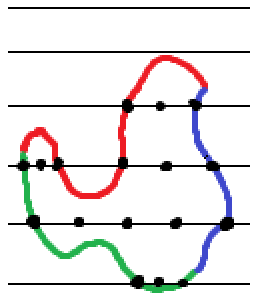
\includegraphics[width=\columnwidth]{figures/raycasting_quadrature}
    \caption{Figure showing how raycasting quadrature works (top), convergence plot for volume integration (bottom}
    \label{fig:raycasting}
\end{figure}

\section{Physics-Based Animation}
Having defined the individual components of the SEM method, we now briefly detail how we apply it to the problem of 
physics-based animation, specifically elastodynamics. 
The advantage of having a unified kinematic description~(\refeq{kinematics}) is that we can directly apply Lagrangian Mechanics~\cite{lanczos2012variational} to arrive at 
the pertinent equations of motion:
\begin{equation*}
    \MM\ddot{\vc{q}} = \fo\left(\vc{q}\right) + \vc{f}_g + \fext,
\end{equation*} where $\MM\in\real^{n\times n}$ is the mass matrix, $\ddot{\vc{q}}\in\real^{n}$ are the generalized accelerations, $\vc{q}\in\real^{n}$ is the stacked vector of surface control points, $\fo\in\real^{n}$ is the 
vector of internal forces, $\vc{f}_g\in\real^{n}$ are body forces such as gravity and $\fext\in\real^{n}$ are external forces such as those due to contact. 
We use penalty springs~\cite{10.1145/1964921.1964932} to resolve contact, and the approach of \citet{10.1145/566654.566623} for approximating frictional effects. 
Because SEM yields equations of motion in the standard form, it is compatible with any standard integration scheme, though in this submission we limit ourselves to
Implicit Euler.

\begin{algorithm}[h]
	\begin{algorithmic}[1]
		\Procedure{Preprocess}{$model$}
     	\myworries{todo: add volume}
     	\While {$simulating$}
     		\State{$\Pcox \gets \Pi\mathbf{q}$}
     		\ForAll{$i \gets 1$ to $|\st{X}|$}
     			\State{$\mathbf{F}_i \gets \frac{\partial \mathbf{F}}{\partial c} c$}
				\State{$\frac{\partial V}{\partial c} \gets \frac{\partial V}{\partial c} +
				\frac{\partial \mathbf{F}}{\partial c}^T \frac{\partial \psi}{\partial \mathbf{F}}(\mathbf{F}_i)$}
				
				\State{$\frac{\partial^2 V}{\partial c^2} \gets \frac{\partial^2 V}{\partial c^2} +
				 \frac{\partial \mathbf{F}}{\partial c}^T 
				 \frac{\partial^2 \psi}{\partial \mathbf{F}^2}(\mathbf{F}_i)
				 \frac{\partial \mathbf{F}}{\partial c}
				 $}
  			\EndFor
  			\State{$K \gets \Pi^T \frac{\partial^2 V}{\partial c^2} \Pi$}
  			\State{$f_{\text{internal}} \gets \Pi^T \frac{\partial V}{\partial c}$}
  			\State{$f_{\text{error}} \gets \ME \vc{q}$}
  			\State{$f_{\text{total}} \gets f_{\text{internal}} + f_{\text{error}} + f_{\text{ext}}$}
  			\State{$\dot{\mathbf{q}} \gets \text{TimeIntegration}
  			(f_{\text{total}},\mathbf{K}, \dot{\mathbf{q}}, \mathbf{J} , \mathbf{M}, \mathbf{M_E})$}
  			\State{$\mathbf{q} \gets \mathbf{q} + h\dot{\mathbf{q}}$}
     	\EndWhile
	\EndProcedure
\end{algorithmic}
\caption{Shape Matching Element Simulation Loop}
\label{alg:sem_simulation}
\end{algorithm}

\subsection{Generalized Velocity}

We can rewrite \refeq{kinematics} in matrix form as 

\begin{equation}
    \defX\left(\refX\right) = \shapef\left(\refX\right)\bldmat\Pi\vc{q},
\end{equation} where $\shapef\in\real^{3\times n} = \begin{bmatrix}P_1\left(\refX\right) \dots P_m\left(\refX\right)\end{bmatrix}$, $m$ is number of 
parts in the object, $\bldmat$ is the diagonal matrix of blending weights and $\Pi$ is the global projection operator.

The velocity of a point on the object is then  
\begin{equation}
        \vc{v}\left(\refX\right) = \underbrace{\shapef\left(\refX\right)\bldmat\Pi}_{\Jkin}\dot{\vc{q}},
    \end{equation} where $\Jkin\left(\refX\right)$ is the kinematic Jacobian and $\dot{\vc{q}}$ are the generalized velocities of the system.

\subsection{Mass Matrix}
\label{ssec:mass_matrix}

We derive the mass matrix for our system from the definition of kinetic energy:
\begin{equation}
    T = \frac{1}{2}\dot{\vc{q}}^T\underbrace{\Pi^T\int_{\Omega}\bldmat\left(\refX\right)^T\shapef\left(\refX\right)^T\shapef\left(\refX\right)\bldmat\left(\refX\right)d\Omega\Pi}_{\MM}\dot{\vc{q}},
\end{equation}
% \begin{equation}
% T = \frac{1}{2}\int_{ \Omega} \rho \dot{\mathbf{x}}^T\dot{\mathbf{x}} d\Omega
% \text{,}
% \end{equation}
% where $\Omega$ is the 3D integration domain, $\rho$ is the density, and $\dot{\mathbf{x}}$ is the velocity for some point in the domain. Using the deformation map defined in \ref{eqn:compact_x_map}, we may rewrite this kinetic energy as
% \begin{equation}
% \begin{split}
% T & = \frac{1}{2}\int_{ \Omega} \rho \dot{\mathbf{q}}^T \mathbf{J}^T\mathbf{Y(X)}^T\mathbf{Y(X)}\ d\Omega \\
%   & = \frac{1}{2} \dot{\mathbf{q}}^T \mathbf{J}^T \left[ \int_{ \Omega} \rho \mathbf{Y(X)}^T\mathbf{Y(X)} d\Omega \right] \mathbf{J}\dot{\mathbf{q}} \\
%   & = \frac{1}{2} \dot{\mathbf{q}}^T \mathbf{M} \dot{\mathbf{q}}
% \end{split}
% \text{.}
% \end{equation}
% The second line is a result of the fact that all terms except for $\mathbf{Y(X)}$ are spatially constant, allowing us to move these outside the volume integral, which enables fast assembly of the mass matrix, $\mathbf{M}$.


\subsection{Deformation Gradient}
The deformation at a point $\refX$ in the reference space is given by
\begin{equation}
    \frac{\partial\defX}{\partial \refX} = \sum_{i=1}^m\left(\bld_i\frac{\partial \Pmatxi}{\partial X}\Pi_i\vc{q}_i + \frac{\partial \bld_i}{\partial X}\Pmatxi\Pi_i\vc{q}\right), 
\end{equation}

For physics-based animation, we find that it is sufficient to assume the blending weights are constant in the region around quadrature points, allowing us to discard the second term.
% \dave{gotta deal with this weight gradient}
% At this point we have shown how to fit a polynomial describing the deformation of each surface. With these polynomial coefficients coupled with their associated centers of mass, we can construct an estimate of some arbitrary material point $\mathbf{X}$ using the deformation described by the surface. This lends itself to a general definition for the deformed position of a point as a weighted sum of the polynomials, which yields a unique polynomial for the point. Thus we arrive at a definition for the deformed position, $\mathbf{x}$, of a material point $\mathbf{X}$ in the undeformed space:
% \begin{equation}
% \label{eqn:deformation_map}
% 	\mathbf{x}(\mathbf{X}) = \sum_i^n w_i(\mathbf{X}) \left[ \mathbf{M}(\mathbf{X-\bar{X}}_j)\mathbf{c}_i + \mathbf{t}_j \right]
% 	\text{,}
% \end{equation}
% where we have $n$ surfaces, and $w_i$ and $\mathbf{c}_i$ are the weights and the coefficients for the $i$-th surface, respectively. The terms $\mathbf{\bar{X}}_j$ and $\mathbf{t}_j$ the undeformed and deformed centers of mass, respectively, that are associated with the $i$-th surface.

\subsection{Constitutive Models}
Our algorithm supports arbitrary elastic constitutive models. 
In this submission we focus on hyperelastic models~\cite{10.1145/2343483.2343501} wherein the potential energy stored by the object, per unit volume,
is given by the strain energy density function $\psi\left(\defo\right)$, and its internal forces and stiffness are the negative gradient and hessian respectively. 
Evaluating and applying constitutive models of this form requires the ability to (1) evaluate the deformation gradient over the reference domain of the model and 
(2) integrate the resulting constitutive properties. 
SEM provides both features and thus support for such models.

\subsection{External Forces}
We compute the force of gravity and apply external forces in the standard way.
Gravity is defined as $\vc{f}_g = \int_{\Omega} \rho\vc{g} d\Omega$, where $\vc{g}$ is the acceleration due to gravity acting on the object. 
We leverage our meshless quadrature~(\refsec{quadrature}) for integration.

External point forces are applied using the Jacobian transpose technique which specifies that the generalized force, $\fext$, 
that results from a point load, applied at $\refX$ is given by $\fext=\Jkin^T\vc{f}\left(\refX\right)$, where $\vc{f}$ is the point load itself.
Using the Jacobian transpose allows us to easily apply all manner of external forces including collision and frictional forces. 

\subsection{Error Energy}
\label{ssec:error_energy}
Like all VEM-type methods, ours requires an error energy to ensure its consistency~\cite{10.1142/S021820251440003X}.
A natural choice is to adapt the error energy specified by \citet{10.1145/1073204.1073216} to penalize deviations between the pose prescribed by  $\vc{q}$ and 
that prescribed by polynomial basis. 

The total error at the boundary of the object can be written as
\begin{equation}
\epsilon = \int_{\partial\Omega}||\Gamma\left(\refX\right)\vc{q} - \Jnurbs\left(\refX\right)\vc{q}||_2^2 d\refX, \\
\end{equation} which is a quadratic.

We augment our physical system with the  quadratic penalty energy $\gamma\epsilon$ and use it to derive additional force and Hessian terms.
In practice we find that choosing $\gamma $ to be the Young's Modulus of the elastic solid provides good behavior in all cases.
If the polynomial basis can exactly match the deformation of the boundary representation, this error naturally elides to zero.

In the next section we show a plethora of physics-based animations created using our approach.
%%% ------- OLD STUFF BELOW --------
% \section{Methods}
% \dave{We should probably put some pseudo code for the preprocessing and the runtime algorithms right up fron, along with a quick textual walk through of the method.}
% Given a volumetric model composed of one or more NURBS surfaces, the surface of each surface is reconstructed using a set of control points $\textbf{p}$ and their associated weights $w$. Following D-NURBS \cite{10.1145/176579.176580}, we take our degrees of freedom (DOF) to be control points of the surfaces and produce displacements directly on these control points at each simulation step. We note that we used a simplified version of D-NURBS in which the weights are held constant throughout the simulation and find this not to be limiting \myworries{(feel like we'll need better justification than saying just this?)}. We represent the degrees of freedom for the $i$-th NURBS surface with $m$ control points as $\mathbf{q}_i = \left[ \mathbf{p}_1^T, \dots, \mathbf{p}_m^T \right]^T \in \mathbb{R}^{3m}$. From this definition, we write the DOF for the entire model as $\mathbf{q} = \left[ \mathbf{q}_i^T, \dots, \mathbf{q}_n^T \right]^T$ where $n$ is the number of NURBS surfaces for the model. 

% To evaluate the volumetric integrals in solid mechanics models, we require material points $\mathbf{X} \in \mathbb{R}^{3m}$ in the undeformed space that serve as integration points. Our shape matching element method enables us to evaluate the deformed positions of the material points strictly using positions defined on the boundary. Like in VEM, we fit a polynomial to each boundary primitive (NURBS in this case) describing its deformation. The fitting of these polynomials closely follows that of the Shape Matching \cite{10.1145/1073204.1073216} approach where we perform a least squares polynomial fit to the deformed boundary points. These boundary points are represented by sampled positions on each NURBS surface. Since each surface is associated with a single polynomial, we can construct a unique polynomial for some arbitrary point by blending these polynomials. Thus given some material point $\mathbf{X}_i$ we find it's corresponding deformed position $\mathbf{x}_i$ via a weighted combination of the polynomials. This permits us to build a general deformation map which we use to construct our equations of motion.

% In the following sections, we will first review the simplified D-NURBS model used to form our generalized coordinates. We then present our shape matching algorithm for fitting polynomials to surfaces .... In section ... we next describe how to blend these surface polynomials to construct a general deformation map for material points. Section ... describes our strategy for selecting integration points in the volume through a raycasting approach. Finally, we formulate our equations of motions from a Lagrangian formulation.

% \section{D-NURBS Model}
% \myworries{TODO: Most of these matrices should be paranthesis matrices}
% We provide a brief overview of the D-NURBS formulation presented in \cite{10.1145/176579.176580}. Our models in our method are composed of a collection of NURBS surfaces. 

% \subsection{D-NURBS Formulation}
% A point on a NURBS surface is typically expressed in the following form
% \begin{equation}
% \label{eqn:nurbs_srf}
%     \mathbf{x}(u,v) = \frac{\sum_{i=1}^{n}\sum_{j=1}^{m}  \mathbf{p}_{i,j} w_{i,j} B_{i,k}(u)B_{j,l}(v)}
%     {\sum_{i=1}^{n}\sum_{j=1}^{m} w_{i,j} B_{i,k}(u)B_{j,l}(v)}
%     \text{,}
% \end{equation}
% where where have a total of $nm$ control points $\mathbf{p}$ and weights $w$. Using the B-spline basis functions and the weighted control points, this formula gives a map from our parametric coordinates $u,v$ to their corresponding position on the surface in $\mathbb{R}^{3m}$. $B_{i,k}(u)$ is the B-spline basis function for the $i-th$ control point with degree $k-1$.

% We would like our generalized coordinates to be the control points of the model so that the dynamics operates directly on the original representation. Therefore, we would like to rewrite equation \ref{eqn:nurbs_srf} in the form
% \begin{equation}
%     \mathbf{x}(u,v) = \mathbf{J}(u,v)\mathbf{q}
%     \text{,}
% \end{equation}
% where $\mathbf{q} = \left[ \mathbf{p}_{1,1}^T, \dots, \mathbf{p}_{i,j}^T, \dots, \mathbf{p}_{n,m}^T \right]^T \in \mathbb{R}^{3nm}$ is the set of $nm$ control points \myworries{in the overview I just write $n$ control points, but here i'm writing $nm$} for a single NURBS surface arranged as a column vector. $\mathbf{J} \in  \mathbb{R}^{3 x 3nm}$ is the NURBS jacobian that maps $(u,v)$ coordinates to world positions in $\mathbb{R}^{3}$.

% The NURBS jacobian, $\mathbf{J}$, is a matrix composed of horizontally concatenated $3x3$ blocks where the $(i,j)$-th block is $\frac{\partial \mathbf{x}}{\partial \mathbf{p}_{i,j}}$ for the $(i,j)$-th control point. $\frac{\partial \mathbf{x}}{\partial \mathbf{p}_{i,j}}$ is a diagonal $3x3$ matrix where each diagonal entry $N_{i,j}(\mathbf{u})$ takes the form

% \begin{equation}
% \label{eqn:jacobian_diagonal}
%     N_{i,j}(u,v)
%     = \frac{w_{i,j} B_{i,k}(u)B_{j,l}(v)}{\sum_{i=1}^{n}\sum_{j=1}^{m} w_{i,j} B_{i,k}(u)B_{j,l}(v)}
%     \text{.}
% \end{equation}
% Thus the NURBS jacobian for a single $(u,v)$ pair is written as
% \begin{equation}
% \label{eqn:uv_jacobian}
%     \mathbf{J}(u,v) =
%     \left[ \frac{\partial \mathbf{x}}{\partial \mathbf{p}_{1,1}} \dots
%            \frac{\partial \mathbf{x}}{\partial \mathbf{p}_{i,j}} \dots 
%            \frac{\partial \mathbf{x}}{\partial \mathbf{p}_{n,m}}
%     \right]
%     \text{.}
% \end{equation}

% This formulation is a simplification of the full D-NURBS described in \cite{10.1145/176579.176580} the weights of the NURBS are fixed throughout the simulation. Permitting the dynamics to modify weights would likely improve the expressiveness of the kinematics, but we find fixing the weights affords sufficiently expressive results and improves performance. The performance improvement is a result of having fixed $N_{i,j}(u,v)$ entries over the course of the simulation. The full D-NURBS model requires rebuilding the jacobian and consequently the mass matrices at each time step. 

% \subsection{Generalized Coordinates for a NURBS model}
% The above formulation describes developing the map from a single $(u,v)$ coordinate to its corresponding position on the surface. In our simulation we represent the entire boundary of the NURBS model, so we require samples along each surface. We emphasize that we only require an initial selection of $(u,v)$ coordinates across each surface and the dynamics of the simulation modifies the set of control points $\mathbf{q}$ to modify the world space maps $\mathbf{x}(u,v)=\mathbf{J}(u,v)\mathbf{q}$.

% Let's say for a NURBS surface on the model the DOF column vector is $\mathbf{q}_i$, which is the subset of control points in the generalized coordinates for the $i$-th surface. For a given surface with $m$ pairs of $\mathbf{u}=(u,v)$ coordinates sampled in parametric space, we write the jacobian for the $i$-th surface as \myworries{(should I use something like $\hat{\mathbf{J}}$ instead?)}
% \begin{equation}
% \label{eqn:surface_jacobian}
%     \mathbf{J}_i =
%     \left[ \mathbf{J}(\mathbf{u})_1^T \dots \mathbf{J}(\mathbf{u})_m^T \right]^T
%     \text{.}
% \end{equation}
% Then if $\mathbf{x}_i$ is the set of $m$ world space positions for the $i$-th surface, we may write $\mathbf{x}_i = \mathbf{J}_i \mathbf{q}_i$. Finally, given the full set of generalized coordinates $\mathbf{q} = \left[ \mathbf{q}_i^T, \dots, \mathbf{q}_n^T \right]^T$ with $n$ surfaces, we may write jacobian $\mathbf{J}$ for the entire model as a block diagonal matrix:
% \begin{equation}
% \mathbf{J} = \left[ \begin{array}{ccccc}
% \mathbf{J}_1 &  &  &  &  \\
%  & \ddots &  &  &  \\
%  &  & \mathbf{J}_i & &  \\
%  &  &  & \ddots &  \\
%  &  &  &  & \mathbf{J}_n \\
% \end{array} \right]
% \text{.}
% \end{equation}
% With this equation, the full set of world positions of the NURBS model may be written as $\mathbf{x} = \mathbf{J}\mathbf{q} \in \mathbb{R}^{3N}$ where $N$ is the total number of $(u,v)$ coordinates.


% \subsection{Shape Matching with Multiple Elements}

% \subsection{Computing the Blending Weights}


% \subsection{Generalized Inertia}



% \subsection{Time Integration}
% 